%% start of file `moderncv_ntrp_template_en.tex'.
%% Copyright 2007 Xavier Danaux (xdanaux@gmail.com).
%
% This work may be distributed and/or modified under the
% conditions of the LaTeX Project Public License version 1.3c,
% available at http://www.latex-project.org/lppl/.
%
% Modded by ntrp (nitropowered@gmail.com)
% Modded by PritvhviRaj Narendra

\documentclass[11pt,a4paper]{moderncv}

% moderncv themes
%\moderncvtheme[blue]{casual}                 % optional argument are 'blue' (default), 'orange', 'red', 'green', 'grey' and 'roman' (for roman fonts, instead of sans serif fonts)
\moderncvtheme[green]{classic}                % idem

\usepackage[T1]{fontenc}
% character encoding
\usepackage[utf8x]{inputenc}                  

%\usepackage{tgpagella}
%\renewcommand{\sfdefault}{\rmdefault}

\definecolor{lightgreen}{rgb}{0.7,1,0.7}

\usepackage{eso-pic}
\AddToShipoutPictureBG{%
	\AtPageLowerLeft{ 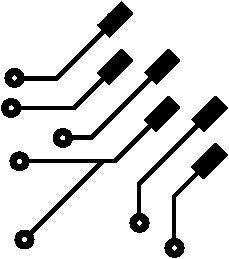
\includegraphics[scale=0.6]{PCB_corner.pdf}}}


\usepackage[savepos]{zref}% http://ctan.org/pkg/zref
\makeatletter
\@ifundefined{zsaveposx}{\let\zsaveposx\zsavepos}{}
\newcounter{hposcnt}
\renewcommand*{\thehposcnt}{hpos\number\value{hposcnt}}
\newcommand*{\tab}[2]{% \tab{<len>}{<stuff>}
	\stepcounter{hposcnt}%
	\zsaveposx{\thehposcnt}%
	\zref@refused{\thehposcnt}%
	\kern\dimexpr-\zposx{\thehposcnt}sp+1in+\oddsidemargin\relax%
	\rlap{\kern#1\relax#2}%
	\kern\dimexpr-1in-\oddsidemargin+\zposx{\thehposcnt}sp\relax%
}

% adjust the page margins
\usepackage[scale=0.86]{geometry}
\recomputelengths                             
% required when changes are made to page layout lengths

\fancyfoot{} % clear all footer fields
\fancyfoot[LE,RO]{\thepage}           % page number in "outer" position of footer line
\fancyfoot[RE,LO]{\footnotesize } % other info in "inner" position of footer line

\renewcommand*{\quotestyle}[1]{{\quotefont\textcolor{color0}{#1}}}
\renewcommand*{\titlestyle}[1]{{\titlefont\textcolor{color2}{#1}}}

\renewcommand*{\recomputecvlengths}{%
	\setlength{\quotewidth}{0.93\textwidth}
}	

% personal data
\firstname{PrithviRaj}
\familyname{Narendra}
\title{Curriculum Vitae}               % optional, remove the line if not wanted
\address{Ringslebenstrasse 2}{Berlin 12353, Germany}    % optional, remove the line if not wanted
\mobile{+49-15758311202}                    % optional, remove the line if not wanted
%\phone{<Phone number>}                      % optional, remove the line if not wanted
%\fax{<Fax number>}                          % optional, remove the line if not wanted
\email{prithvirajnarendra@gmail.com}                      % optional, remove the line if not wanted
%\extrainfo{additional information (optional)} % optional, remove the line if not wanted
%\photo[84pt]{placeholder.jpg}                         % '64pt' is the height the picture must be resized to and 'picture' is the name of the picture file; optional, remove the line if not wanted
\quote{I'm a geek. I cherish contributing and using Open Source technology. I care about sustainability and conservation of the environment. I am proficient with embedded systems and lean iterative development cycle of designing, prototyping and testing.}% \textbf{TODO based on application}}                 % optional, remove the line if not wanted

%\nopagenumbers{}                             % uncomment to suppress automatic page numbering for CVs longer than one page


\newcommand{\leftRatingIndent}{48ex}
\newcommand{\rightRatingIndent}{105ex}

%----------------------------------------------------------------------------------
%            content
%----------------------------------------------------------------------------------
\begin{document}
\maketitle



%Section
\section{\textbf{Desidered Employment}}
\cvline{}{\normalsize I am looking to join an organization where I am able to use my technical and entrepreneurial skills for social and/or environmental betterment.}


%Section
\section{\textbf{Skills}} 
\subsection{Hardware}
\cvcomputer{PCB Design}{GeDA, Eagle, OrCAD, KiCad, Altium} {Electronics}{Circuit Design \tab{\rightRatingIndent}{\large \textcolor{color1}{•••••}}
	\newline Digital Design \tab{\rightRatingIndent}{\large \textcolor{color1}{••••}\textcolor{lightgreen}{•}}
	\newline Analog Design \tab{\rightRatingIndent}{\large \textcolor{color1}{••}\textcolor{lightgreen}{•••}}}
\vspace{-15px}
\cvcomputer{Hands-On}{SMD soldering, analog \& digital debugging} {}{}
\subsection{Software}

\cvcomputer{Languages}{C, Embedded-C \tab{\leftRatingIndent}{\large \textcolor{color1}{•••••}}
	 \newline Python, bash scripting, C++ \tab{\leftRatingIndent}{\large \textcolor{color1}{•••}\textcolor{lightgreen}{••}}
	 \newline HTML, Java, C\#, Assembly \tab{\leftRatingIndent}{\large \textcolor{color1}{••}\textcolor{lightgreen}{•••}}} 
	{Protocols}{BLE, I2C, UART, SPI \tab{\rightRatingIndent}{\large \textcolor{color1}{•••••}}
	 \newline CAN, Ethernet \tab{\rightRatingIndent}{\large \textcolor{color1}{•••}\textcolor{lightgreen}{••}}
	 \newline USB, 6LowPAN \tab{\rightRatingIndent}{\large \textcolor{color1}{••}\textcolor{lightgreen}{•••}}}

\cvcomputer{Tools}{Eclipse, GCC, Keil, IAR, Android Studio, Git, Doxygen, \LaTeX}  {Know-how}{$\mu$C optimized coding, sensor/actuator interfacing, power optimization, algorithm to embedded firmware development }

%Section

\section{\textbf{Experience}}
\subsection{Working}
\cventry{Nov 2014\newline{to}\newline{Apr 2015}}{Firmware Engineer}{\href{http://bluvision.com/}{BluVision}}{Berlin}{}{I mainly worked developing firmware for the CC2650 Chip, which drives the Bluetooth Low Energy (BLE) Beacons by BluVision. Specifically, I interfaced a light and motion detection sensors, developed the complete Host Controller Interface (HCI) layer and developed firmwares for customer specific applications. I also developed Android apps to configure beacons and log advertisements.  I've got an idea of Design for Manufacturing (DFM) in both hardware and software, with experience in a factory in China. Finally, It was a good experience learning the do's and don'ts when managing a start-up. } % arguments 3 to 6 are optional

\cventry{Oct 2011 - Jul 2012}{Research Assistant - Wildlife Researchers' Gadgets Maker}{\newline \href{http://www.dese.iisc.ernet.in/}{Department of Electronic Systems Engineering}, Indian Institute of Science}{Bangalore}{}{Being the project assistant for Dr. André Pittet I was involved in the complete product design cycle of fabricating gadgets such as camera traps and animal collars for wildlife researchers, which had specific requirements such as low cost, ruggedness and weeks of battery life. My tasks included features decision, design, implementation and testing of the enclosure (3D modelling), electronics (PCB schematics, routing and soldering) and software (embedded software, windows PC application, android application).} % arguments 3 to 6 are optional

\subsection{Academic}
\cventry{Jan 2014 -- Sep 2014}{Master Thesis - Comparison of link layer of BLE and 802.15.4}{\newline \href{https://www.sics.se/groups/networked-embedded-systems-group-nes}{Swedish Institute of Computer Science}}{Stockholm}{}{The objective of my thesis was firstly to port Contiki OS and Bluetooth Low Energy (BLE) Protocol to a SoC platform that supports BLE and secondly to compare various performance criteria such as data rate, latency, and energy consumption with 802.15.4 based MAC layers (ContikiMAC and Null-RDC). A demo of the Contiki port was also showcased. } % arguments 3 to 6 are optional

\cventry{Sep 2013 -- Jan 2014}{Member, MicroGrid Project 2013}{\href{https://tta-portal.misc.kth.se/microgrid}{Technology Transfer Alliance}}{KTH}{Stockholm}{In this project we designed a 2nd generation a MicroGrid network intended to create a local power network in rural and remote regions. This network consisted of a central server managing an efficient MicroGrid of distributed DC-DC converters nodes with CoAP messages. The function of these node units running on Contiki-OS was to keep the voltage steady within the central grid while using heterogeneous power sources such as solar energy, batteries and super-capacitors.}

\subsection{Projects}
\cventry{Aug 2010 -- June 2011}{Team Leader}{\href{http://www.teamstudsat.in/}{Project STUDSAT-2}}{Bangalore}{}{STUDSAT-2 is the 2\textsuperscript{nd} generation satellite project by students from many colleges across India. As team leader of STUDSAT-2, I had both technical and management roles. My major tasks included conducting management meets, recruiting students, preparing the project timeline and presenting in various organizations to raise funds for the project. My technical work was focused on the use of Real Time Operating System's (FREE-RTOS) features for satellite applications and developing a prototype of the checkout system. In addition, I led the process of analyzing and selecting the payload and core controller for the satellite and interfacing the on and off chip peripherals.}

\cventry{Feb 2009 -- June 2010}{Team Member}{\href{http://www.teamstudsat.in/}{Project STUDSAT-1}}{Bangalore}{}{In this project, I developed the electronics and software for the CMOS camera payload for this nano-satellite, using a 0.3 Mega-Pixel Monochrome Kodak sensor to take images of 95 m resolution. I also was part of the team that developed a simple scheduler based Operating System for the satellite.} % arguments 3 to 6 are optional

%Section
\section{\textbf{Education}}
\cventry{Sep 2012 -- Sep 2014}{\href{http://www.masterschool.eitictlabs.eu/}{Masters in EIT ICT Labs Master School}}{}{\newline Major in \emph{\href{http://www.masterschool.eitictlabs.eu/programmes/es/}{Embedded Systems}}, Minor in \emph{\href{http://www.masterschool.eitictlabs.eu/programmes/minor/}{Innovation and Entrepreneurship}}}{}{Year 1: \emph{\href{http://tue.nl/}{Technische Universiteit Eindhoven}}, Einhoven, Netherlands\newline Year 2: \emph{\href{https://www.kth.se/en}{KTH Royal Institute of Technology}}, Stockholm, Sweden} % arguments 3 to 6 are optional

\cventry{Sep 2007 -- May 2011}{Bachelors in Electronics and Communication}{\href{http://rvce.edu.in/}{RV College of Engineering}}{Banglaore}{}{Best Outgoing Student Award from the Electronics \& Communication Dept. for the 2007-11 batch.} % arguments 3 to 6 are optional

%Section
\section{\textbf{Additional Experience/Volunteer}}
\cventry{Feb 2015 -- Present}{Event Officer}{\href{http://alumni.eitictlabs.eu/}{EIT ICT Labs Alumni Board}}{}{}{Primary task of facilitating and supporting creation of events by the Alumni and current students.}

\cventry{Sep 2009 -- May   2010}{Secretary}{IEEE RVCE Chapter}{}{}{Apart from being a secretary, I was organized paper presentations and robotics workshops}

\cventry{}{Volunteer/Member}{Miscellaneous groups and organizations}{}{}{Was secretary at \href{https://www.gewis.nl/~scifi/}{SCIFI}, TU Eindhovem for 6 months; volunteered for 8 months at a NGO to help children at a school for visually impaired; organized many events in a student group called `Geekopreneurs' in KTH for 6 months.}

\section{\textbf{Interests and Hobbies}}
\cvline{}{Playing badminton, following technological updates, watching TED and other talks which makes me ponder, listening to music, reading fiction, watching movies, trekking, and traveling.}

%Section
\section{\textbf{Further Info}}
\cvcomputer{Citizenship}{\small Indian\normalsize}{Birth}{\small 20/09/1989\normalsize}
%\cvline{Birth}{\small 20/09/1989 \normalsize}
%\cvline{Elance}{\small \url{<Link to profile>}\normalsize}
\cvcomputer{LinkedIn}{\small \url{linkedin.com/in/prithvirajnarendra}\normalsize}{Github}{\small \url{github.com/EarthLord}\normalsize}
\cvcomputer{References}{\small In the LinkedIn page} {CouchSurfing}{\url{couchsurfing.com/people/prithvirajnarendra}}
%\cvline{Blog}{\small \url{<Link to profile>}\normalsize}
%\cvline{Skype}{\small <skype>\normalsize}

\end{document}